%iffalse
\let\negmedspace\undefined
\let\negthickspace\undefined
\documentclass[journal,12pt,onecolumn]{IEEEtran}
\usepackage{cite}
\usepackage{amsmath,amssymb,amsfonts,amsthm}
\usepackage{algorithmic}
\usepackage{graphicx}
\usepackage{textcomp}
\usepackage{xcolor}
\usepackage{txfonts}
\usepackage{listings}
\usepackage{enumitem}
\usepackage{mathtools}
\usepackage{gensymb}
\usepackage{comment}
\usepackage[breaklinks=true]{hyperref}
\usepackage{tkz-euclide} 
\usepackage{listings}
\usepackage{gvv}                                        
%\def\inputGnumericTable{}                                 
\usepackage[latin1]{inputenc}                                
\usepackage{color}                                            
\usepackage{array}                                            
\usepackage{longtable}                                       
\usepackage{calc}                                             
\usepackage{multirow}                                         
\usepackage{hhline}                                           
\usepackage{ifthen}                                           
\usepackage{lscape}
\usepackage{tabularx}
\usepackage{array}
\usepackage{float}


\newtheorem{theorem}{Theorem}[section]
\newtheorem{problem}{Problem}
\newtheorem{proposition}{Proposition}[section]
\newtheorem{lemma}{Lemma}[section]
\newtheorem{corollary}[theorem]{Corollary}
\newtheorem{example}{Example}[section]
\newtheorem{definition}[problem]{Definition}
\newcommand{\BEQA}{\begin{eqnarray}}
\newcommand{\EEQA}{\end{eqnarray}}
\newcommand{\define}{\stackrel{\triangle}{=}}
\theoremstyle{remark}
\newtheorem{rem}{Remark}

% Marks the beginning of the document
\begin{document}
\bibliographystyle{IEEEtran}
\vspace{3cm}

\title{1-1.6.16}
\author{AI24BTECH11011 - Himani Gourishetty}
\maketitle
\bigskip

\renewcommand{\thefigure}{\theenumi}
\renewcommand{\thetable}{\theenumi}
\begin{enumerate}
\item Find the values of k if the points $\vec{A}\brak{k+1,2k}$ , $\vec{B}\brak{3k,2k+3}$ , $\vec{C}\brak{5k-1,5k}$ are collinear.\\
\textbf{Solution} Given,\\
\begin{table}[h!]    
\centering
\begin{tabular}[12pt]{ |c|c|c|}
\hline
\textbf{Variable} & \textbf{Description} & \textbf{formula}\\ 
\hline
$\vec{A}\brak{x1,y1}$ & $\brak{k+1,2k}$  & - \\
\hline 
$\vec{B}\brak{x2,y2}$ & $\brak{3k,2k+3}$ & - \\
\hline
$\vec{C}\brak{x3,y3}$ & $\brak{5k-1,5k}$ & - \\
\hline 
Area & Area formed by the 3 points & $x1\brak{y2-y3}+x2\brak{y3-y1}+x3\brak{y1-y2}\\
\hline
\end{tabular}

\label{q3}
\end{table}\\
for these points to be collinear , the area should be zero;
\begin{align}
Area = x1(y2-y3)+x2(y3-y1)+x3(y1-y2)\\
0 = \brak{k+1}\brak{-3k+3}+\brak{3k}\brak{3k}+\brak{5k-1}\brak{-3}\\
0 = 6k^2-15k+6
0 = \brak{6k-3}\brak{k-2}
\end{align}
then, 
\begin{align}
k=2;
k=0.5   
\end{align}
\begin{figure}[ht]
   \centering
   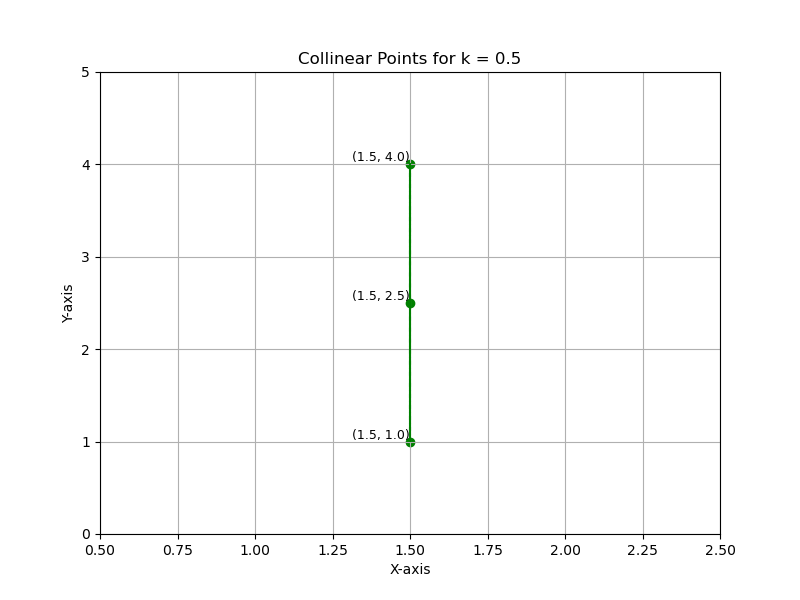
\includegraphics[width=0.7\linewidth]{figs/q3_1.png}
   \label{q31}
\end{figure}
\begin{figure}[ht]
   \centering
   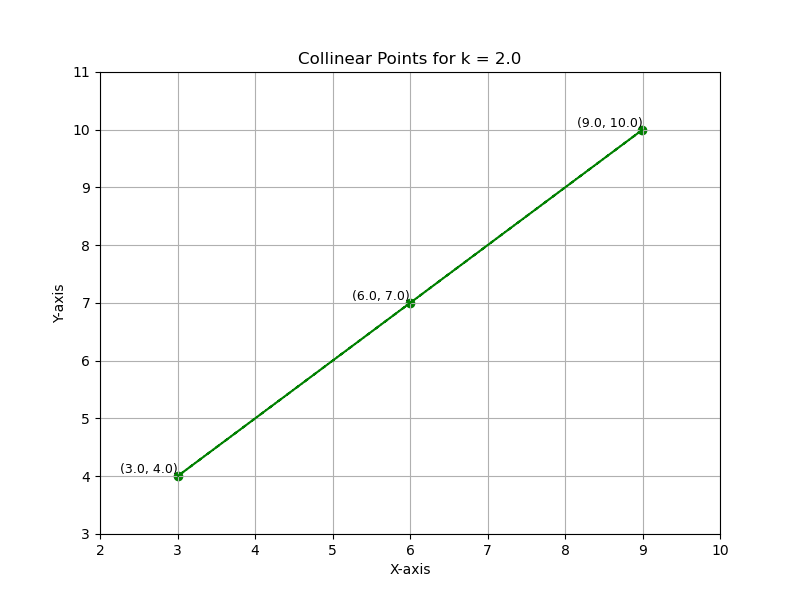
\includegraphics[width=0.7\linewidth]{figs/q3_2.png}
   \label{q32}
\end{figure}

\end{document}
